\begin{frame}
\begin{center}
\Huge{Functions, modules, classes, exceptions and plotting}
\end{center}
\end{frame}

\begin{frame}
    \begin{center}
    \Huge{Functions}
    \end{center}
\end{frame}

\begin{frame}[fragile]
    \frametitle{Functions}
Defining a function which returns a Fibonacci series up to n.
    \begin{myColorBox}{0.9}{}
\begin{verbatim}
>>> def fib(n):
...     """Return the Fibonacci series up to n."""
...     result = []
...     a, b = 0, 1
...     while a < n:
...         result.append(a)
...         a, b = b, a+b
...     return result
\end{verbatim}
    \end{myColorBox}
\pause
Now call the function we just defined:
    \begin{myColorBox}{0.9}{}
\begin{verbatim}
>>> fib(100)
[0, 1, 1, 2, 3, 5, 8, 13, 21, 34, 55, 89]
\end{verbatim}
    \end{myColorBox}
\end{frame}

\begin{frame}[fragile]
    \frametitle{Functions}
    \begin{myColorBox}{0.9}{}
\begin{verbatim}
def birthday2(name, age = 1):
    msg = "Happy birthday, %s! You're %d today."
    print  msg % (name, age)
\end{verbatim}
    \end{myColorBox}
\pause
    \begin{myColorBox}{0.9}{}
\begin{verbatim}
>>> birthday2("Katherine")
Happy birthday, Katherine! You're 1 today.
\end{verbatim}
    \end{myColorBox}
\pause
    \begin{myColorBox}{0.9}{}
\begin{verbatim}
>>> birthday2(age = 12, name = "Katherine")
Happy birthday, Katherine! You're 12 today.
\end{verbatim}
    \end{myColorBox}
\pause
    \begin{myColorBox}{0.9}{}
\begin{verbatim}
>>> birthday2("Katherine", 14)
Happy birthday, Katherine! You're 14 today.
\end{verbatim}
    \end{myColorBox}
\end{frame}

\begin{frame}
    \begin{center}
    \Huge{Modules}
    \end{center}
\end{frame}

\begin{frame}[fragile]
    \frametitle{Modules}
Importing functionality of a module the normal and safe way:
    \begin{myColorBox}{0.9}{}
\begin{verbatim}
>>> import math
>>> math.pi
3.141592653589793
>>> math.cos(math.pi)
-1.0
\end{verbatim}
    \end{myColorBox}
\pause
Importing directly into the local namespace:
    \begin{myColorBox}{0.9}{}
\begin{verbatim}
>>> from math import *
>>> pi
3.141592653589793
>>> cos(pi)
-1.0
\end{verbatim}
    \end{myColorBox}
\end{frame}

\begin{frame}[fragile]
\frametitle{Modules}
Caution with \verb#from module import *#
    \begin{myColorBox}{0.9}{}
\begin{verbatim}
>>> from os import *
>>> f = open('Makefile','r')
Traceback (most recent call last):
  File "<stdin>", line 1, in <module>
TypeError: an integer is required

# open() has been mapped to os.open() !!!
\end{verbatim}
\end{myColorBox}
The builtin open() could still be accessed though:
\begin{myColorBox}{0.9}{}
\begin{verbatim}
>>> f = __builtins__.open('Makefile','r')
\end{verbatim}
\end{myColorBox}
\end{frame}

\begin{frame}[fragile]
\frametitle{Modules}
Less typing while avoiding collisions by binding to local names
\begin{myColorBox}{0.9}{}
\begin{verbatim}
>>> import math
>>> cos = math.cos
>>> pi = math.pi
>>> cos(pi)
-1.0
\end{verbatim}
\end{myColorBox}

Import module under a different/shorter name:
\begin{myColorBox}{0.9}{}
\begin{verbatim}
>>> import math as m
>>> m.cos(m.pi)
-1.0
\end{verbatim}
\end{myColorBox}

Import only what is needed:
\begin{myColorBox}{0.9}{}
\begin{verbatim}
>>> from math import pi, cos
>>> cos(pi)
-1.0
\end{verbatim}
\end{myColorBox}
\end{frame}

\begin{frame}[fragile]
\frametitle{Modules}
Writing your own module called \verb#seismo.py#:
\begin{verbatim}
"""Some seismological utility functions."""

import math

def lame_parameters(alpha, beta, density):
    """ Convert seismic velocities to Lame's parameters.
        Returns Lame's parameters as (lambda, mu)."""
    return ((alpha ** 2 - 2.0 * beta ** 2) * density,
            beta ** 2 * density)

def velocities(lambd, mu, density):
    """ Convert lame parameters to seismic velocities.
        Returns tuple with velocities (alpha, beta). """
    return (math.sqrt((lambd + 2.0 * mu) / density),
            math.sqrt(mu / density))
\end{verbatim}
\end{frame}

\begin{frame}[fragile]
\frametitle{Modules}
Using your module as any other module:
\begin{myColorBox}{0.9}{}
\begin{verbatim}
>>> import seismo
>>> seismo.lame_parameters(4000., 2100., 2600.)
(18668000000.0, 11466000000.0)
>>> _
(18668000000.0, 11466000000.0)
>>> (_+(2600,))
(18668000000.0, 11466000000.0, 2600)
>>> seismo.velocities(*(_+(2600,)))
(4000.0, 2100.0)
\end{verbatim}
\end{myColorBox}
\end{frame}

\begin{frame}[fragile]
\frametitle{Modules}
Help!
\begin{myColorBox}{1.0}{}
\begin{verbatim}
>>> import seismo
>>> help(seismo)
\end{verbatim}
\end{myColorBox}
\begin{myColorBox}{1.0}{}
\begin{verbatim}
Help on module seismo:

NAME
    seismo - Some seismological utility functions.

FILE
    /obspy_git/branches/docs/sed_2012/seismo.py

FUNCTIONS
    lame_parameters(alpha, beta, density)
        Convert seismic velocities to Lame's parameters.
        Returns Lame's parameters as (lambda, mu).
    
    velocities(lambd, mu, density)
        Convert lame parameters to seismic velocities.
        Returns tuple with velocities (alpha, beta).

\end{verbatim}
\end{myColorBox}
\end{frame}

\begin{frame}[fragile]
\frametitle{Modules}
You can look at the contents of any module
\begin{myColorBox}{0.9}{}
\begin{verbatim}
>>> import seismo
>>> dir(seismo)
['__builtins__', '__doc__', '__file__', 
'__name__', '__package__', 'lame_parameters', 
'math', 'velocities']

\end{verbatim}
\end{myColorBox}
\verb#dir# without argument looks at local namespace
\begin{myColorBox}{0.9}{}
\begin{verbatim}
... 
>>> dir()
['__builtins__', '__doc__',
 '__name__', '__package__', 'seismo']
\end{verbatim}
\end{myColorBox}
\end{frame}

\begin{frame}
    \begin{center}
    \Huge{Errors and Exceptions}
    \end{center}
\end{frame}

\begin{frame}[fragile]
    \frametitle{Errors and Exceptions}
    \begin{myColorBox}{1.0}{}
\begin{verbatim}
>>> 10 * (1/0)
Traceback (most recent call last):
  File "<stdin>", line 1, in ?
ZeroDivisionError: integer division or modulo by zero
\end{verbatim}
    \end{myColorBox}
    \pause    
    \begin{myColorBox}{1.0}{}
\begin{verbatim}
>>> 4 + muh*3
Traceback (most recent call last):
  File "<stdin>", line 1, in ?
NameError: name 'muh' is not defined
\end{verbatim}
    \end{myColorBox}
    \pause    
    \begin{myColorBox}{1.0}{}
\begin{verbatim}
>>> '2' + 2
Traceback (most recent call last):
  File "<stdin>", line 1, in ?
TypeError: cannot concatenate 'str' and 'int' objects
\end{verbatim}
    \end{myColorBox}
\end{frame}


\begin{frame}[fragile]
    \frametitle{Errors and Exceptions}
Handling Exceptions:
    \begin{myColorBox}{1.0}{}
\begin{verbatim}
def divide(x, y):
    try:
        result = x / y
    except ZeroDivisionError:
        print "division by zero!"
    except TypeError:
        print "unsupported type!"
    else:
        print "result is", result
\end{verbatim}
    \end{myColorBox}
    \begin{myColorBox}{1.0}{}
\begin{verbatim}
>>> divide(2, 1)
result is 2
>>> divide(2, 0)
division by zero!
>>> divide(2, 'bbb')
unsupported type!
\end{verbatim}
    \end{myColorBox}
\end{frame}

\begin{frame}[fragile]
\frametitle{Errors and Exceptions}
More generic Exception handling:
\begin{myColorBox}{1.0}{}
\begin{verbatim}
def divide(x, y):
    try:
        result = x / y
    except Exception, e:
        print "Generic exception! ", e
    else:
        print "result is", result
\end{verbatim}
\end{myColorBox}
    \begin{myColorBox}{1.0}{}
    \begin{verbatim}
>>> divide(3.,'blub')
Generic exception!  unsupported operand type(s) 
for /: 'float' and 'str'

>>> divide(3.,0)
Generic exception!  float division by zero
 
\end{verbatim}
\end{myColorBox}
\end{frame}

\begin{frame}
    \begin{center}
    \Huge{Classes}
    \end{center}
\end{frame}


\begin{frame}[fragile]
    \frametitle{Classes}
    Classes consist of..
    \begin{itemize}
    \item Attributes: Variables that store information about the class' current
    state
    \item Methods: Functions that allow interactions with the class
    \end{itemize}
    Some advantages of using classes..
    \begin{itemize}
    \item Classes know how to behave by themselves
    \item Users do not need to know the details of the class implementation
    \item Programs using the classes get shorter and far more readable
    \end{itemize}
\end{frame}

\begin{frame}[fragile]
\frametitle{Classes}
Syntax:
\begin{itemize}
  \item The \verb#class# keyword introduces a class
  \item To create an instance of the class, use function notation
  \item The \verb#__init__()# method is invoked when an instance of the class is
  created
  \item Class methods receive a reference to the instance as first argument. By
  convention it is called \verb#self#
  \item An \textit{instance object} is an entity encapsulating state (data
  attributes) and behaviour (methods)
  \item A \textit{class} is the blueprint from which individual objects
  (\textit{instances}) are created.
\end{itemize}
\end{frame}

\begin{frame}[fragile]
    \frametitle{Classes}
Example:
    \begin{myColorBox}{0.9}{}
\small
\begin{verbatim}
class Rectangle:
    def __init__(self,x,y):
        self.x = x
        self.y = y

    def area(self):
        return self.x * self.y
\end{verbatim}
    \end{myColorBox}
    \begin{myColorBox}{0.9}{}
\small
\begin{verbatim}
>>> r = Rectangle(10,20)
>>> r.area()
200
\end{verbatim}
    \end{myColorBox}
\end{frame}

\begin{frame}[fragile]
\frametitle{Classes}
Inheritance
\begin{itemize}
  \item Motivation: add functionality but reuse existing code
  \item A derived class has all the attributes and methods from the base class
  but can add new attributes and methods
  \item If any new attributes or methods have the same name as an attribute or
  method in the base class, it is used instead of the base class version.
  \item The syntax is simply \verb#class DerivedClass(BaseClass): ...#
\end{itemize}
\end{frame}

\begin{frame}[fragile]
\frametitle{Classes}
Example:
\begin{myColorBox}{0.9}{}
\begin{verbatim}
class Square(Rectangle):
    def __init__(self,x):
        self.x = x
        self.y = x
\end{verbatim}
\end{myColorBox}
\begin{myColorBox}{0.9}{}
\begin{verbatim}
>>> s = Square(5)
>>> s.area()
25
\end{verbatim}
\end{myColorBox}
\end{frame}

\begin{frame}
    \begin{center}
    \Huge{Plotting}
    \end{center}
\end{frame}

\begin{frame}[fragile]
    \frametitle{Plotting}
Matplotlib is \emph{the} plotting library for Python.
\begin{itemize}
\item syntax is close to Matlab's plotting commands
\item advanced users can control all details of the plots
\end{itemize}
We need to import \verb#matplotlib# for the following examples:
\begin{myColorBox}{0.9}{}
\begin{verbatim}
>>> import matplotlib.pyplot as plt
>>> x = [0, 2, 2.5]
>>> plt.plot(x)
[<matplotlib.lines.Line2D object at 0x3372e10>]
>>> plt.show()
\end{verbatim}
    \end{myColorBox}
\pause
\begin{center}
      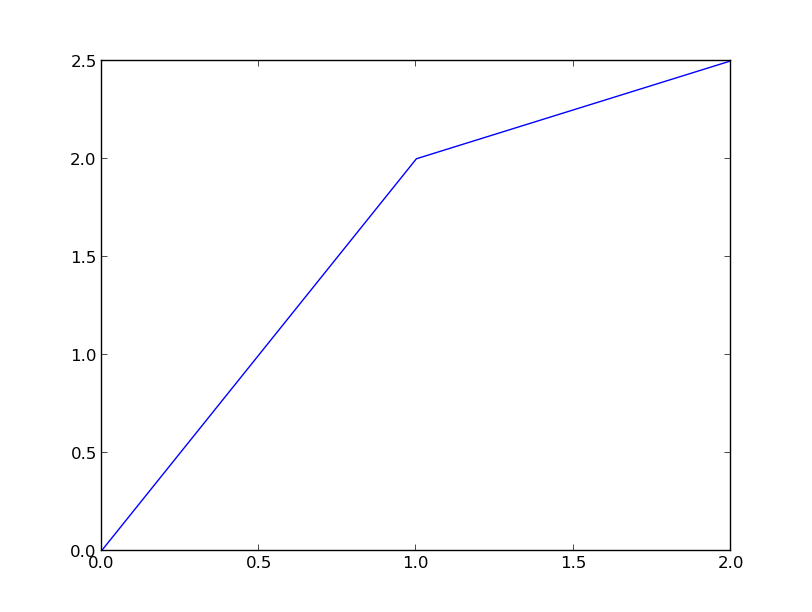
\includegraphics[width=0.4\textwidth]{pix/matplotlib_example_1}
    \end{center}
\end{frame}

\begin{frame}[fragile]
	\frametitle{Plotting}
    \begin{myColorBox}{0.9}{}
\begin{verbatim}
>>> x = [0, 2, 2.5]
>>> y = [1, 2.5, 3.5]
>>> plt.plot(x, y, 'ro')
>>> plt.xlim(-1, 3)
>>> plt.ylim(0, 4)
>>> plt.show()
\end{verbatim}
    \end{myColorBox}
\pause
\begin{center}
      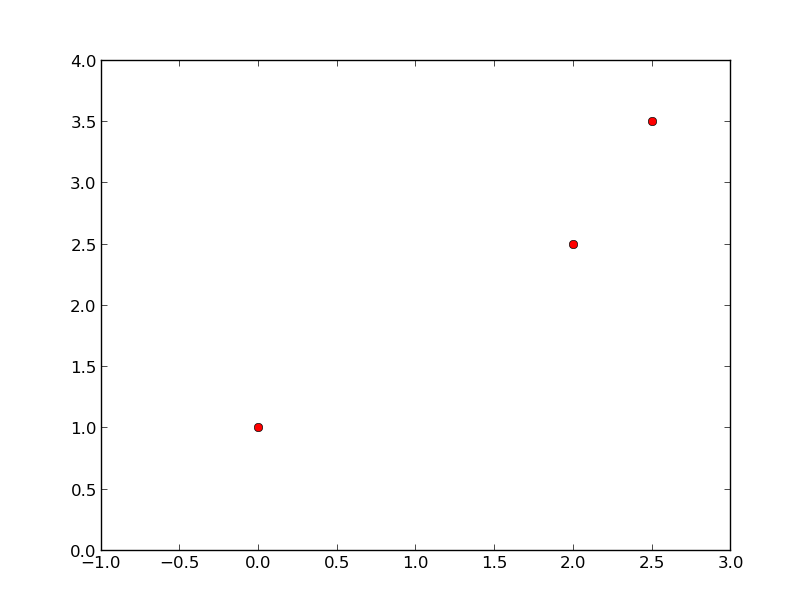
\includegraphics[width=0.6\textwidth]{pix/matplotlib_example_2}
\end{center}
\end{frame}

\begin{frame}[fragile]
    \frametitle{Plotting}
    \begin{myColorBox}{0.9}{}
\begin{verbatim}
>>> import math
>>> t = [0.1 * i for i in range(0,20)]
>>> s = [math.sin(2*math.pi*x) for x in t]
>>> plt.plot(t, s, linewidth=1.0)
>>> plt.xlabel('time (s)')
>>> plt.ylabel('voltage (mV)')
>>> plt.title('This is a very simple plot')
>>> plt.grid(True)
>>> plt.show()
\end{verbatim}
    \end{myColorBox}
\pause
\begin{center}
      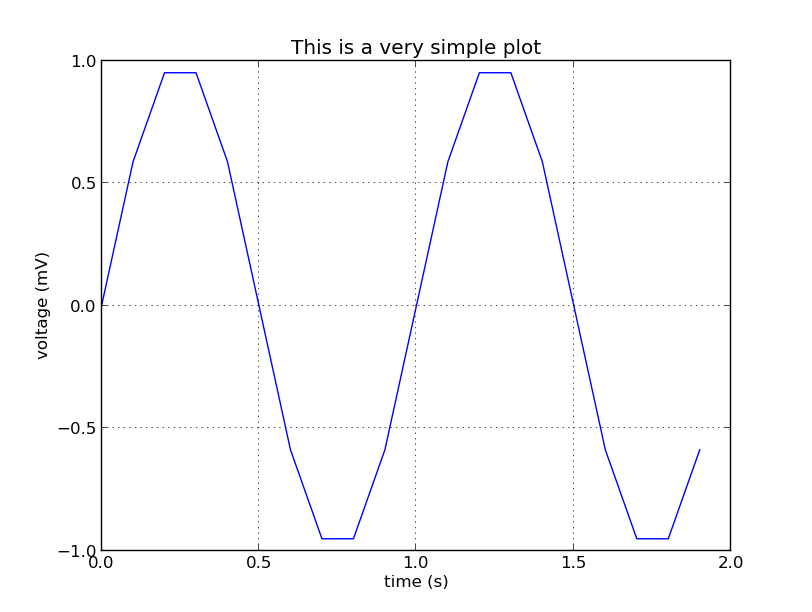
\includegraphics[width=0.5\textwidth]{pix/matplotlib_example_3}
\end{center}
\end{frame}

\begin{frame}
\frametitle{Plotting}
See the Matplotlib homepage for basic plotting commands and especially the
Matplotlib Gallery for many plotting examples with source code!\\
\href{http://matplotlib.sourceforge.net/index.html}{http://matplotlib.sourceforge.net/index.html}
\href{http://matplotlib.sourceforge.net/gallery.html}{http://matplotlib.sourceforge.net/gallery.html}
\end{frame}

\begin{frame}
\begin{center}
\Huge{Exercises}
\end{center}
\end{frame}

